% !TEX root = ../beamer.tex
\section{Manufacturing Ecosystem Evolution}
\subsection{Evolution Aim \& Main Factors}
\begin{frame}{Envolving Aim \& Main Factors}{Manufacturing Ecosystem Envolving}
\only<1-2>{The evolution  aim in the Ecosystem is to: \begin{itemize}
\item optimize the utilize of manufacturing resources
\item find the adaptive operating model for enterprises
\item filter out the undesirable enterprises.
\end{itemize}}
\only<2>{
\begin{block}{Main Factors for Evolution}
\begin{itemize}
\item Rating Schema;
\item Recommand System;
\item Criterion of User Introduction and Elimination
\end{itemize}
\end{block}}
\only<3>{
	\begin{figure}\centering
		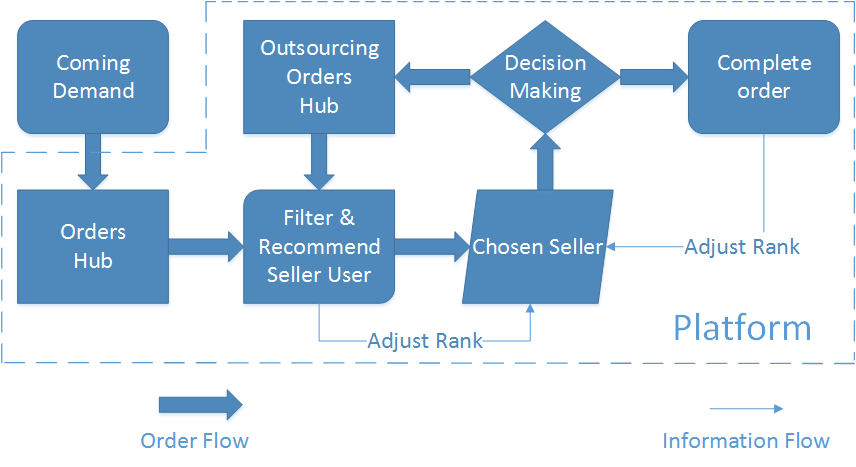
\includegraphics[width =\textwidth]{figures/wanting.png}
		\caption{The Ideal Model of the System}
	\end{figure}
}
\end{frame}

\subsection{Rating Schema}
\begin{frame}{Rating Schema}{Manufacturing Ecosystem Envolving}
\onslide<+->{Rating user's rank is the base of Recommand System, so the rating schema should be designed. Most modern rating systems are derived from Elo's model}
\onslide<+->{\begin{numcases}{}
E_A = \frac{1}{1+10^{\frac{R_B-R_A}{400}}} \\
R_A := R_A + K(S_A - E_A) \\
E_B = \frac{1}{1+10^{\frac{R_A-R_B}{400}}} \\
R_B := R_B + K(S_B - E_B)
\end{numcases}}
\end{frame}

\subsection{Recommand System}
\begin{frame}{Recommandation System}{Manufacturing Ecosystem Evolution}
\onslide<+->{There are two scenarios in recommendation:
\begin{itemize}
\item Service Searching
\item Platform priority setting
\end{itemize}
}
\onslide<+->{
	Collaboration Filtering is a popular method used in recommand system:
	\begin{equation}
	\begin{split}
	\min_{p_*,q_*,b_*} & \sum_{(u,i)\in\kappa}\left(r_{ui} -\mu - b_u - b_i - p^T_uq_i \right)^2 \\
		& + \lambda_3 \left( \|p_u\|^2 + \|q_i\|^2 + b_u^2 + b_i^2 \right)
	\end{split}
	\end{equation}
	\begin{numcases}{}
	\hat{r}_{ui} = b_{ui} + p^T_uq_i \\
	b_{ui} = \mu + b_u + b_i  \\
	\kappa =\{(u,i)|r_{ui} \text{is known}\}
	\end{numcases}
}
\end{frame}

\subsection{User Introduction \& Elimination}
\begin{frame}{User Introduction \& Elimination}{Manufacturing Ecosystem Envolving}
\onslide<+->{
	Ecosystem envolving need a good user introduction and elimination method with:
}
\onslide<+->{
	\begin{block}{Evolution}
	\begin{itemize}
	\item Reinforcement Learning
	\item Control
	\end{itemize}
	\end{block}
}
\end{frame}

\subsection{Envision of the Ecosystem}
\begin{frame}{Envision}{After a long running time and the system seems stable}
\onslide<+->{
	With poper scheduling and evolution, Cloud Manufacturing Ecosystem running with a stable mode:
	\begin{block}{Stable System Envision}
	\begin{itemize}
		\item Less-Popular manufacturing services are utilization instead of idleness with Coupon
		\item Products are manufactured with appropriate resources
		\item High rank users in different types of manufacturing resource lead the industrial chain
		\item Good operating models improved with time goes by
	\end{itemize}
	\end{block}
}
\end{frame}


\subsection{Simple Demo} % (fold)
\label{sub:simple_demo}
\begin{frame}{Simple Demo}
\only<1>{
Based on Elo model, we focus on the how sellers' ranks will
change with different specifications.

If we set $Q_A=10^{\frac{R_A}{400}}$ and $Q_B=10^{\frac{R_B}{400}}$, we have:
$$
\begin{cases}
E_A = \frac{Q_A}{Q_A + Q_B}\\
E_B = \frac{Q_B}{Q_B + Q_A}
\end{cases}
$$}
\only<2>{
For entity in the ecosystem(seller) $i,k$ ($i,k=1,2,\dots,n$), we assume that:
$$
\begin{cases}
Q_A = Q_i\\
Q_B = \frac{\sum_{k}\alpha_{ik}Q_k}{\sum_{k}\alpha_{ik}}
\end{cases}
$$
Where $\alpha_{ik}$ is the threating coefficient, the bigger the values is, the heigher $k$ threatens $i$.

\begin{center}
\href{localhost:8888}{\large Demo}
\end{center}
}
\end{frame}
% subsection simple_demo (end)
\iffalse
\subsection{Reinforcement Learning and Control} % (fold)
\label{sub:reinforcement_learning_and_control}
\begin{frame}{Aim}{Reinforcement Learning}
\begin{block}{The aim}
\begin{itemize}
	\item Uncover the right action for user
	\item Uncover the right action for administrator to make adjustments
	\item From the view of user
	\item From the view of industrial chain
\end{itemize}
\end{block}
\end{frame}

\begin{frame}{Main Parts}{Reinforcement Learning}
\begin{block}{Main parts and steps}
\begin{itemize}
	\item Define states
	\item Design actions
	\item Set reward function
	\item Design state simulation
	\item Simulate
\end{itemize}
\end{block}
\end{frame}
\fi
